\documentclass{article}
\usepackage{hyperref}
\usepackage{Style}

\nocite{*} % Comentar si quiero citar
%\addbibresource{bibliografia.bib} % Quitar el comentado si quiero usar bibliografia

\begin{document}

\begin{minipage}{2.5cm}
    \includegraphics[width=2cm]{imagen_puc.jpg}
\end{minipage}
\begin{minipage}{14cm}
    {\sc Pontificia Universidad Católica de Chile\\
    Facultad de Matemáticas\\
    Departamento de Matemática\\
    Profesora: Amal Taarabt -- Estudiante: Benjamín Mateluna}
\end{minipage}
\vspace{1ex}

{\centerline{\bf Teoría Espectral - MAT2820}
\centerline{\bf Tarea 1}}
\centerline{\bf 15 de septiembre de 2025}

\section{Transformada de Fourier - Versión continua}
\subsection{Propiedades básicas}
\begin{enumerate}
    \item Veamos que para todo $\xi\in\R$ se tiene que $\abs{\F(f)(\xi)}<\infty$, en efecto,
    \begin{equation*}
        \abs{\int_{\R}e^{-ix\xi}f(x)\hspace{1mm}dx}\leq\int_{\R}\abs{e^{-ix\xi}f(x)}\hspace{1mm}dx
        =\int_{\R}\abs{f(x)}\hspace{1mm}dx<\infty
    \end{equation*}
    donde la última desigualdad se obtiene de que $f\in L^{1}(\R)$. Lo anterior implica que 
    $\hat{f}(\xi)\in\C$.

    \item En primer lugar, se tiene que
    \begin{align*}
        \F(g_{1})(\xi) &= \frac{1}{\sqrt{2\pi}}\int_{\R}e^{-ix\xi}e^{-\abs{x}}\hspace{1mm}dx
        =\frac{1}{\sqrt{2\pi}}\int_{\R}e^{-ix\xi-\abs{x}}\hspace{1mm}dx
        =\frac{1}{\sqrt{2\pi}}\left(\int_{\R_{\geq0}}e^{-x-ix\xi}\hspace{1mm}dx
        +\int_{\R_{\leq0}}e^{x-ix\xi}\hspace{1mm}dx\right) \\[2mm]
        &= \frac{1}{\sqrt{2\pi}}\left(-\frac{e^{-x(1+i\xi)}}{1+i\xi}\Big|_{x=0}^{\infty}
        +\frac{e^{x(1-i\xi)}}{1-i\xi}\Big|_{-\infty}^{x=0}\right)
        =\frac{1}{\sqrt{2\pi}}\cdot\frac{2}{1+\xi^{2}}
    \end{align*}

    \vspace{2mm}
    Por otro lado, para $g_{2}$, definimos la función compleja $f:\C\to\C$ dada por
    \begin{equation*}
        f(z)=\frac{e^{-iz\xi}}{1+z^{2}}
    \end{equation*}
    Supongamos que $\xi\leq0$, consiramos el siguiente camino en $\C$,
    \begin{center}
        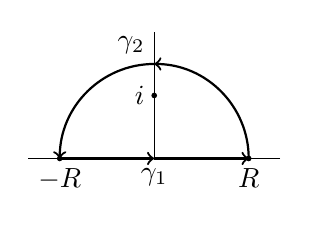
\begin{tikzpicture}[scale=0.8] %Dominio de integración
            \draw[thick, ->] (1.5,0) arc (0:90:1.5);
            \draw[thick, ->] (0,1.5) arc (90:180:1.5);
            
            \coordinate (O) at (0,0);
            \coordinate (A) at (2,0);
            \coordinate (B) at (-2,0);
            \coordinate (C) at (0,2);

            \draw (A) -- (B);
            \draw (O) -- (C);

            \draw[thick, ->] (-1.5,0) -- (0,0);
            \draw[thick, ->] (0,0) -- (1.5,0);

            \filldraw (0,1.5) node[anchor=south east]{$\gamma_{2}$};
            \filldraw (0,0) node[anchor=north]{$\gamma_{1}$};
            \filldraw (-1.5,0) circle (1pt) node[anchor=north]{$-R$};
            \filldraw (1.5,0) circle (1pt) node[anchor=north]{$R$};

            \filldraw (0,1) circle (1pt) node[anchor=east]{$i$};
        \end{tikzpicture}
    \end{center}
    donde $\gamma_{1}(t)=t$ con $t\in[-R,R]$ y $\gamma_{2}(t)=Re^{\pi it}$ para $t\in[0,1]$. 
    Diremos que $\gamma=\gamma_{1}+\gamma_{2}$. Para $R>1$ suficientemente grande se tiene que 
    $i$ esta en la región determinada por $\gamma$, así, por teorema del residuo, se sigue que
    \begin{equation*}
        2\pi i\cdot Res(f,i)=\int_{\gamma}f(z)\hspace{1mm}dz=\int_{\gamma_{1}}f(z)\hspace{1mm}dz
        +\int_{\gamma_{2}}f(z)\hspace{1mm}dz=\int_{-R}^{R}\frac{e^{-it\xi}}{1+t^{2}}\hspace{1mm}dt
        +\int_{0}^{1}\frac{e^{-iRe^{i\pi t}\xi}}{1+R^{2}e^{2\pi it}}\cdot Ri\pi e^{i\pi t}
        \hspace{1mm}dt
    \end{equation*}
    como $i$ es un polo simple de $f$, vemos que
    \begin{equation*}
        Res(f,i)=\lim\limits_{z\to i}(z-i)f(z)=\lim\limits_{z\to i}\frac{e^{-iz\xi}}{z+i}
        =-\frac{i}{2}e^{\xi}
    \end{equation*}
    Por otro lado, como $\xi\leq0$, tenemos que
    \begin{align*}
        \abs{\int_{0}^{1}\frac{e^{-iRe^{i\pi t}\xi}}{1+R^{2}e^{2\pi it}}\cdot Ri\pi e^{i\pi t}
        \hspace{1mm}dt}\leq\int_{0}^{1}\frac{R\pi e^{Rsen(\pi t)\xi}}{\abs{1+R^{2}e^{2\pi it}}}
        \hspace{1mm}dt\leq\int_{0}^{1}\frac{R\pi}{R^{2}-1}\hspace{1mm}dt
        =\frac{R\pi}{R^{2}-1}\xrightarrow[R\to\infty]{}0
    \end{align*}
    Entonces para $\xi\leq0$ se tiene que
    \begin{equation*}
        \F(g_{2})(\xi)=\frac{1}{\sqrt{2\pi}}\int_{\R}\frac{e^{-ix\xi}}{1+x^{2}}\hspace{1mm}dx
        =\frac{\pi}{\sqrt{2\pi}}e^{\xi}
    \end{equation*}
    De manera análoga para $\xi>0$, pero tomando $\gamma_{2}(t)=Re^{-\pi it}$ con $t\in[0,1]$, se 
    obtiene que
    \begin{equation*}
        \F(g_{2})(\xi)=-\frac{\pi}{\sqrt{2\pi}}e^{-\xi}
    \end{equation*}
    
    \item Consideremos la función
    \begin{equation*}
        G(x,\xi)=e^{-ix\xi}\cdot e^{-\frac{x^{2}}{2}}=e^{-(ix\xi+\frac{x^{2}}{2})}
    \end{equation*}
    notemos que $g_{\xi_{0}}(x)=G(x,\xi_{0})$ es continua, por ende es medible, también se tiene 
    que $\pdv{G}{\xi}$ existe para todo $(x,\xi)\in\R^{2}$ y además $g_{0}(x)$ es integrable.
    Veamos que
    \begin{equation*}
        \abs{\pdv{G}{\xi}(x,\xi)}\leq e^{-\frac{x^{2}}{2}}\in L^{1}(\R)
    \end{equation*}
    Así, derivando bajo el signo de la integral se obtiene que
    \begin{align*}
        (\F(f))'(\xi) &= \frac{-i}{\sqrt{2\pi}}\int_{\R}xe^{-\frac{x^{2}}{2}}
        e^{-ix\xi}\hspace{1mm}dx=\frac{-i}{\sqrt{2\pi}}\left(-e^{-\frac{x^{2}}{2}}e^{-ix\xi}
        \Big|_{-\infty}^{\infty}-i\xi\int_{\R}e^{-\frac{x^{2}}{2}}e^{-ix\xi}\hspace{1mm}dx
        \right) \\[2mm]
        &= \frac{-\xi}{\sqrt{2\pi}}\F(f)(\xi)
    \end{align*}
    Nos queda una EDO de variables separables con condición inicial $\F(f)(0)=1$, resolviendo la 
    ecuación resulta que
    \begin{equation*}
        \F(f)(\xi)=e^{-\frac{\xi^{2}}{2}}
    \end{equation*}
    
    \item (Reescribir)
    Supongamos que $f$ es indicatriz de algún $E\subseteq\R$ medible, luego,
    \begin{equation*}
        \F(f)(\xi)=\int_{\R}f(x)e^{-ix\xi}\hspace{1mm}dx=\int_{E}e^{-ix\xi}\hspace{1mm}dx
    \end{equation*}
    Supongamos que $E=I=(a,b)$ donde $a<b$, entonces
    \begin{equation*}
        \F(f)(\xi)=\int_{a}^{b}e^{-ix\xi}\hspace{1mm}dx=-\frac{e^{-ix\xi}}{i\xi}\Big|_{a}^{b}
        =\frac{e^{-ia\xi}}{i\xi}-\frac{e^{-ib\xi}}{i\xi}\xrightarrow[\abs{\xi}\to+\infty]{}0
    \end{equation*}
    Para una colección finita de intervalos disjuntos de a pares el resultado es inmediato, este
    se puede extender a una colección numerable de intervalos disjuntos de a pares. Sea 
    $O\subseteq\R$ un conjunto abierto, luego, se escribe como unión numerable de intervalos 
    disjuntos de a pares, entonces
    \begin{equation*}
        \F(\I_{O})(\xi)\xrightarrow[\abs{\xi}\to+\infty]{}0
    \end{equation*}
    Sea $E$ un conjunto medible, sea $\varepsilon>0$, existe $G\supseteq E$ abierto tal que 
    $\lambda(G\setminus E)<\varepsilon$, entonces
    \begin{equation*}
        \abs{\int_{G}e^{-ix\xi}\hspace{1mm}dx-\int_{E}e^{-ix\xi}\hspace{1mm}dx}
        =\abs{\int_{G\setminus E}e^{-ix\xi}\hspace{1mm}dx}\leq\lambda(G\setminus E)<\varepsilon
    \end{equation*}
    lo que implica que
    \begin{equation*}
        \abs{\lim\limits_{\abs{\xi}\to+\infty}\int_{E}e^{-ix\xi}\hspace{1mm}dx}\leq\varepsilon
    \end{equation*}
    para todo $\varepsilon>0$, se sigue que
    \begin{equation*}
        \lim\limits_{\abs{\xi}\to+\infty}\int_{E}e^{-ix\xi}\hspace{1mm}dx=0
    \end{equation*}
    Sea $s\in L^{1}(\R)$ una función simple, el resultado es directo, en efecto,
    \begin{equation*}
        \lim\limits_{\abs{\xi}\to+\infty}\F(s)(\xi)=\lim\limits_{\abs{\xi}\to+\infty}\int_{\R}
        e^{-ix\xi}\sum_{i}a_{i}\I_{A_{i}}\hspace{1mm}dx=\sum_{i}a_{i}
        \lim\limits_{\abs{\xi}\to+\infty}\int_{A_{i}}e^{-ix\xi}\hspace{1mm}dx=0
    \end{equation*}
    Sea $f\in L^{1}(\R)$, entonces existe $(s_{n})_{n}$ tal que $s_{n}\xrightarrow[n\to\infty]{}f$
    en $L^{1}(\R)$, notemos que
    \begin{equation*}
        \abs{\F(f)(\xi)}-\abs{\F(s_{n})(\xi)}\leq\abs{\F(f)(\xi)-\F(s_{n})(\xi)}
        \leq\int_{\R}\abs{f(x)-s_{n}(x)}\hspace{1mm}dx
    \end{equation*}
    Luego, existe $N\in\N$ tal que $\abs{\F(f)(\xi)}$
    
    \item Veamos que es lineal, sean $f,g\in L^{1}(\R)$ y $\alpha\in\C$, entonces por linealidad
    de la intregal, vemos que
    \begin{equation*}
        \F(f+\alpha g)(\xi)=\frac{1}{\sqrt{2\pi}}\int_{\R}e^{-ix\xi}(f+\alpha g)(x)\hspace{1mm}dx
        =\frac{1}{\sqrt{2\pi}}\int_{\R}e^{-ix\xi}f(x)\hspace{1mm}dx
        +\frac{\alpha}{\sqrt{2\pi}}\int_{\R}e^{-ix\xi}g(x)\hspace{1mm}dx
        =\F(f)(\xi)+\alpha\F(g)(\xi)
    \end{equation*}
    Queda ver que $\F$ es continua, sean $f_{n}$ tales que $f_{n}\xrightarrow[]{L^{1}}f$, tenemos 
    que
    \begin{equation*}
        \abs{\F(f)(\xi)-\F(f_{n})(\xi)}=\abs{\F(f-f_{n})(\xi)}
        \leq\frac{1}{\sqrt{2\pi}}\int_{\R}\abs{f-f_{n}}\hspace{1mm}dx\xrightarrow[n\to\infty]{}0
        \htext{para todo }\xi\in\R
    \end{equation*}
    Por lo tanto $\F$ es una aplicación lineal continua. Además, dado $\xi\in\R$ se sigue que
    \begin{equation*}
        \abs{\F(f)(\xi)}\leq\frac{1}{\sqrt{2\pi}}\int_{\R}\abs{f(x)}\hspace{1mm}dx
        =\frac{1}{\sqrt{2\pi}}\norm{f}_{L^{1}}
    \end{equation*}
    es decir, $\norm{\F(f)}_{\infty}\leq\frac{1}{\sqrt{2\pi}}\norm{f}_{L^{1}}$.
    
    \item No se especifica claramente como debería estar bien definida la convolución. 
    Demostraremos que es finita c.t.p y que dadas $f,g\in L^{1}(\R)$ entonces $f*g\in L^{1}(\R)$. 
    En efecto, usando tonelli obtenemos que
    \begin{equation*}
        \int_{\R}\abs{(f*g)(x)}\hspace{1mm}dx
        =\int_{\R}\abs{\int_{\R}f(t)g(x-t)\hspace{1mm}dt}\hspace{1mm}dx
        \leq\int_{\R}\int_{\R}\abs{f(t)g(x-t)}\hspace{1mm}dt\hspace{1mm}dx
        =\int_{\R}\int_{\R}\abs{f(t)}\abs{g(x-t)}\hspace{1mm}dx\hspace{1mm}dt
        =\norm{f}_{L^{1}}\cdot\norm{g}_{L^{1}}
    \end{equation*}
    es decir, $\norm{f*g}_{L^{1}}\leq\norm{f}_{L^{1}}\cdot\norm{g}_{L^{1}}<\infty$, lo que implica
    que $f*g$ es finita c.t.p. Veamos que $\F(f*g)=\sqrt{2\pi}\F(f)\F(g)$, en efecto,
    \begin{align*}
        \F(f*g)(\xi) &= \frac{1}{\sqrt{2\pi}}\int_{\R}e^{-ix\xi}(f*g)(x)\hspace{1mm}dx
        =\frac{1}{\sqrt{2\pi}}\int_{\R}e^{-ix\xi}\int_{\R}f(t)g(x-t)\hspace{1mm}dt\hspace{1mm}dx
        =\frac{1}{\sqrt{2\pi}}\int_{\R}\int_{\R}e^{-ix\xi}f(t)g(x-t)\hspace{1mm}dt\hspace{1mm}dx 
        \\[2mm]
        &= \frac{1}{\sqrt{2\pi}}\int_{\R}\int_{\R}e^{-ix\xi}f(t)g(x-t)\hspace{1mm}dx\hspace{1mm}dt
        =\frac{1}{\sqrt{2\pi}}\int_{\R}\int_{\R}
        e^{-ix\xi}e^{-it\xi}f(t)g(x)\hspace{1mm}dx\hspace{1mm}dt \\[2mm]
        &= \frac{1}{\sqrt{2\pi}}\int_{\R}e^{-it\xi}f(t)\hspace{1mm}dt
        \cdot\int_{\R}e^{-ix\xi}g(x)\hspace{1mm}dx=\sqrt{2\pi}\F(f)\F(g)
    \end{align*}
\end{enumerate}

\newpage
\subsection{Fórmula de inversión}
\begin{enumerate}
    \item Sobre la transformada de Fourier
    \begin{enumerate}
        \item 
        
        \item 
    
    \end{enumerate}
    \item\textbf{Aplicación a la resolución de EDP.}
    \begin{enumerate}
        \item Como $f\in L^{1}(\R)\cap\mathcal{C}^{1}(\R)$ se tiene que 
        $\lim_{\abs{x}\to\infty}f(x)=0$, luego integrando por partes obtenemos que
        \begin{equation*}
            \F\left(\pdv{f}{x}\right)(\xi)
            =\frac{1}{\sqrt{2\pi}}\int_{\R}e^{-ix\xi}\pdv{f}{x}(x)\hspace{1mm}dx
            =\frac{1}{\sqrt{2\pi}}
            \left(e^{-ix\xi}f(x)\Big|_{-\infty}^{\infty}+i\xi\int_{\R}e^{-ix\xi}f(x)\hspace{1mm}dx
            \right)=i\xi\F(f)(\xi)
        \end{equation*}
        lo que prueba lo pedido.
        
        \item Definimos la función $G(x,\xi)=e^{-ix\xi}f(x)$. La función 
        $g_{\xi_{0}}(x)=G(x,\xi_{0})$ es medible, por que es multiplicación de funciones medibles,
        la derivada parcial de $G$ respecto a $\xi$ existe para todo $(x,\xi)\in\R^{2}$ y 
        $g_{0}(x)$ es integrable. Además,
        \begin{equation*}
            \abs{\pdv{F}{\xi}(x,\xi)}\leq\abs{xf(x)}\in L^{1}(\R)
        \end{equation*}
        Así, derivando bajo el signo de la integral vemos que
        \begin{equation*}
            \pdv{\hat{f}}{\xi}(\xi)
            =\frac{1}{\sqrt{2\pi}}\cdot\pdv{}{\xi}\int_{\R}e^{-ix\xi}f(x)\hspace{1mm}dx
            =\frac{-i}{\sqrt{2\pi}}\int_{\R}e^{-ix\xi}xf(x)\hspace{1mm}dx=-i\F(xf)(\xi)
        \end{equation*}
        lo que concluye el ejercicio.
    
    \end{enumerate}
\end{enumerate}

\newpage
\subsection{La transformada de Fourier en \texorpdfstring{$L^{2}(\mathbb{R})$}{}}

\newpage
\subsection{La transformada de Fourier en \texorpdfstring{$\mathcal{S}(\R)$}{}}
\noindent Sea $f\in S(\R)$.
\begin{lema}
    Sea $g\in L^{1}(\R)$. Entonces $(f*g)^{'}(x)=(f'*g)(x)$.
\end{lema}
\begin{proof}
    la función que mapea $t$ a $F(x,t):=f(x-t)g(t)$ es medible para todo $t\in\R$, la derivada 
    parcial de $F$ respecto a $x$ existe para todo $(x,t)\in\R^{2}$ y como la convolución esta
    bien definida, existe $x_{0}$ tal que $F(x_{0},t)$ es integrable, es decir, 
    $(f*g)(x_{0})<\infty$. Además, observamos que
    \begin{equation*}
        \abs{\pdv{F}{x}(x,t)}=\abs{\pdv{f}{x}(x-t)g(t)}
        \leq\norm{f}_{\infty}\abs{g(t)}\in L^{1}(\R)
        \htext{para todo}t\in\R
    \end{equation*}
    Derivando bajo el signo de la integral, se tiene lo pedido
    \begin{equation*}
        \dv{}{x}(f*g)(x)=\dv{}{x}\int_{\R}f(x-t)g(t)\hspace{1mm}dt
        =\int_{\R}\pdv{f}{x}(x-t)g(t)\hspace{1mm}dt=(f'*g)(x)
    \end{equation*}
\end{proof}

\noindent\textbf{Observación:} Iterando el argumento, llegamos a que $(f*g)^{(n)}(x)$ para 
$(f^{(n)}*g)(x)$ para todo $n\in\N$.

\begin{enumerate}
    \item Sean $f,g\in S(\R)$ y $\alpha\in\C$, dados $k,l\in\N$ tenemos que
    \begin{equation*}
        \sup_{x\in\R}\abs{x^{k}\pdv{^{l}}{x^{l}}(f+\alpha g)}
        =\sup_{x\in\R}\abs{x^{k}\pdv{^{l}f}{x^{l}}+\alpha\cdot x^{k}\pdv{^{l}g}{x^{l}}}
        \leq\sup_{x\in\R}\abs{x^{k}\pdv{^{l}f}{x^{l}}}
        +\abs{\alpha}\cdot\sup_{x\in\R}\abs{x^{k}\pdv{^{l}g}{x^{l}}}<\infty
    \end{equation*}
    Por lo tanto $S(\R)$ es espacio vectorial.

    \item Notemos que
    \begin{align*}
        \phi'(x) &= -2xze^{-zx^{2}} \\
        \phi''(x) &= -2ze^{-zx^{2}}+4x^{2}z^{2}e^{-zx^{2}}
    \end{align*}
    Luego, inductivamente,
    \begin{equation*}
        \phi^{(n)}(x)=\sum_{i=0}^{n}a_{i}x^{i}e^{-zx^{2}}\htext{donde }a_{i}\in\C
    \end{equation*}
    Así, dados $k,l\in\N$
    \begin{equation*}
        \abs{x^{k}\pdv{^{l}\phi}{x^{l}}(x)}=\abs{x^{k}\cdot\sum_{i=0}^{l}a_{i}x^{i}e^{-zx^{2}}}
        \leq\sum_{i=0}^{l}\abs{a_{i}}\abs{x^{i+k}}e^{-Re(z)x^{2}}
        \hhtext{entonces}
        \abs{x^{k}\pdv{^{l}\phi}{x^{l}}(x)}\xrightarrow[\abs{x}\to\infty]{}0
    \end{equation*}
    Donde utilizamos que $Re(z)>0$. Existe $M>0$ tal que $\abs{x^{k}\pdv{^{l}\phi}{x^{l}}(x)}<1$ 
    para todo $x\in\R\setminus[-M,M]$, además, por continuidad y compacidad se sigue que
    \begin{equation*}
        \sup_{x\in[-M,M]}\abs{x^{k}\pdv{^{l}\phi}{x^{l}}}<\infty
    \end{equation*}
    Por lo tanto $\phi\in S(\R)$.
    
    \item Sea $g(x)=\frac{1}{1+x^{2}}$, notemos que para $\abs{x}>1$ se tiene lo siguiente
    \begin{equation*}
        \abs{\frac{x^{3}}{1+x^{2}}}\geq\frac{\abs{x}^{3}}{2\abs{x}^{2}}
        =\frac{\abs{x}}{2}\xrightarrow[\abs{x}\to\infty]{}\infty
    \end{equation*}
    Luego $g\not\in S(\R)$.
    
    \item Sea $\varphi\in C_{c}^{\infty}(\R)$, entonces 
    $K:=\overline{\varphi^{-1}(\R\setminus\{0\})}$ es compacto, además, para $x\in\R\setminus K$ 
    tenemos que
    \begin{equation*}
        x^{k}\pdv{^{l}\varphi}{x^{l}}=0
    \end{equation*}
    para todo $k,l\in\N$, ya que $\overline{\left(\pdv{^{l}\varphi}{x^{l}}\right)^{-1}
    (\R\setminus\{0\})}\subseteq K$. Luego, por continuidad y compacidad, vemos que
    \begin{equation*}
        \sup_{x\in\R}\abs{x^{k}\pdv{^{l}\varphi}{x^{l}}}
        =\sup_{x\in K}\abs{x^{k}\pdv{^{l}\varphi}{x^{l}}}<\infty
    \end{equation*}
    Esto prueba que $C_{c}^{\infty}(\R)\subseteq S(\R)$. Sean $p\geq1$ y $f\in S(\R)$, definimos
    \begin{equation*}
        C:=\sup_{x\in\R}\abs{(1+\abs{x})^{2}f(x)}
    \end{equation*}
    que es finito, ya que $f\in S(\R)$. En particular, se tiene que 
    $C\geq(1+\abs{x})^{2}\abs{f(x)}$ para todo $x\in\R$. Entonces,
    \begin{equation*}
        \int_{\R}\abs{f(x)}^{p}\hspace{1mm}dx\leq\int_{\R}\frac{C^{p}}{(1+\abs{x})^{2p}}
        \hspace{1mm}dx=2C^{p}\int_{\R_{\geq0}}\frac{1}{(1+x)^{2p}}\hspace{1mm}dx
        =2C^{p}\int_{1}^{\infty}\frac{1}{x^{2p}}\hspace{1mm}dx<\infty
    \end{equation*}
    donde lo último se debe a que $2p\geq2$. Si $p=\infty$, como $f$ es continua 
    $\norm{f}_{L^{\infty}}=\sup_{x\in\R}\abs{f}<\infty$. Concluimos que 
    $S(\R)\subseteq L^{p}(\R)$.
    
    \item Debemos probar una serie de propiedades del espacio de Schwartz respecto a algunas 
    operaciones:
    \begin{itemize}
        \item Sea $f\in S(\R)$. Veamos que $S(\R)$ es cerrado bajo derivación, sea $n\in\N$, 
        consideramos $g(x)=f^{(n)}(x)$. Dados $k,l\in\N$ observamos que
        \begin{equation*}
            \sup_{x\in\R}\abs{x^{k}\pdv{^{l}g}{x^{l}}}
            =\sup_{x\in\R}\abs{x^{k}\pdv{^{n+l}f}{x^{n+l}}}<\infty
        \end{equation*}
        lo que prueba que $g\in S(\R)$.

        \item Sea $g\in S(\R)$, afirmamos que $fg\in S(\R)$, en efecto, en 
        primer lugar notemos que
        \begin{equation*}
            \pdv{^{l}}{x^{l}}(fg)(x)
            =\sum_{i=0}^{l}\binom{l}{i}\pdv{^{i}f}{x^{i}}(x)\cdot\pdv{^{l-i}g}{x^{l-i}}(x)
        \end{equation*}
        para todo $l\in\N$, dado $k\in\N$, se sigue que
        \begin{equation*}
            \sup_{x\in\R}\abs{x^{k}\pdv{^{l}}{x^{l}}(fg)}
            \leq\sum_{i=0}^{l}\binom{l}{i}\sup_{x\in\R}\abs{x^{k}\pdv{^{i}f}{x^{i}}}
            \cdot\sup_{x\in\R}\abs{\pdv{^{l-i}g}{x^{l-i}}}<\infty
        \end{equation*}
        donde la última desigualdad se debe a que $f,g\in S(\R)$.

        \item Sea $p\in\C[x]$, luego
        \begin{equation*}
            \sup_{x\in\R}\abs{x^{k}\pdv{^{l}f}{x^{l}}\cdot p}
            \leq\sum_{j=0}^{deg(p)}\abs{a_{i}}\sup_{x\in\R}\abs{x^{k+j}\pdv{^{l}f}{x^{l}}}<\infty
            \hhtext{donde}
            p(x)=\sum_{j=0}^{deg(p)}a_{j}x^{j}
        \end{equation*}
        usando lo probado, la fórmula anterior para la derivada $n-$ésima del producto y que la
        derivada de un polinomio es un polinomio, se obtiene que $fp\in S(\R)$.

        \item Dado $k\in\R$, definimos lo siguiente
        \begin{equation*}
            C_{l}:=\sup_{x\in\R}\abs{x}^{k}\abs{g(x)}<\infty\htext{para}g\in S(\R)
        \end{equation*}
        y para $x,t\in\R$ tenemos la siguiente desigualdad
        \begin{equation*}
            \abs{x}^{k}\leq(\abs{x-t}+\abs{t})^{k}\leq(2\max\{\abs{x-t},{\abs{t}}\})^{k}
            \leq2^{k}\abs{x-t}^{k}+2^{k}\abs{t}^{k}
        \end{equation*}
        Dada $g\in S(\R)$, usando lo anterior, para todo $t\in\R$, vemos lo siguiente
        \begin{equation*}
            \abs{x}^{k}\abs{g(x-t)}\leq2^{k}\abs{x-t}^{k}\abs{g(x-t)}+2^{k}\abs{t}^{k}\abs{g(x-t)}
            \leq2^{k}C_{k}+2^{k}C_{0}\abs{t}^{k}\leq2^{k}(C_{k}+C_{0})(1+\abs{t})^{k}
        \end{equation*}
        Definimos la constante $A_{k}:=2^{k}(C_{k}+C_{0})$. Así, dado $g\in S(\R)$ obtenemos lo 
        siguiente
        \begin{align*}
            \abs{x}^{k}\abs{(f*g)(x)}\leq\int_{\R}\abs{x}^{k}\abs{g(x-t)}\abs{f(t)}\hspace{1mm}dt
            \leq A_{k}\int_{\R}(1+\abs{t})^{k+2}
            \cdot\frac{\abs{f(t)}}{(1+\abs{t})^{2}}\hspace{1mm}dt
            \leq A_{k}\mathcal{C}_{k+2}\int_{\R}\frac{1}{(1+\abs{t})^{2}}\hspace{1mm}dt<\infty
        \end{align*}
        Donde $\mathcal{C}_{k+2}:=\sup_{t\in\R}(1+\abs{t})^{k+2}\abs{f(t)}$ que es finito por que 
        $f\in S(\R)$. Como $g\in S(\R)$ entonces $g^{(l)}\in S(\R)$, usando el mismo argumento y 
        el lema inicial, concluimos que
        \begin{equation*}
            \sup_{x\in\R}\abs{x^{k}\pdv{^{l}}{x^{l}}(f*g)}<\infty\htext{para todo }k,l\in\N
        \end{equation*} 
    \end{itemize}
    
    \item Para $n\in\N$ por lo visto anteriormente resulta que $x^{n}f(x)\in S(\R)$, entonces
    $x^{n}f(x)\to0$ cuando $\abs{x}\to\infty$ y además por el problema 1.2.2.b tenemos una 
    derivada $l-$ésima explícita para $\hat{f}$. Sean $k,l\in\N$, intengrando por partes notamos 
    lo siguiente
    \begin{align*}
        \sqrt{2\pi}\cdot\xi^{k}\pdv{^{l}\hat{f}}{\xi^{l}}(\xi)
        &= \xi^{k}\cdot(-i)^{l}\F(x^{l}f(x))(\xi)
        =\xi^{k}(-i)^{l}\int_{\R}e^{-ix\xi}x^{l}f(x)\hspace{1mm}dx \\[2mm]
        &= \xi^{k}(-i)^{l}\left(i\cdot\frac{e^{-ix\xi}x^{l}f(x)}{\xi}\Big|_{-\infty}^{\infty}
        -\frac{i}{\xi}\int_{\R}e^{-ix\xi}\pdv{}{x}(x^{l}f(x))\hspace{1mm}dx\right) \\[2mm]
        &= \xi^{k-1}(-i)^{l+1}\int_{\R}e^{-ix\xi}\pdv{}{x}(x^{l}f(x))\hspace{1mm}dx=\cdots
        =(-i)^{l+k}\int_{\R}e^{-ix\xi}\pdv{^{k}}{x^{k}}(x^{l}f(x))\hspace{1mm}dx
    \end{align*}
    Como $S(\R)$ es cerrado bajo derivación y multiplicación por un polinomio se tiene que
    \begin{equation*}
        \abs{\xi^{k}\pdv{^{l}\hat{f}}{\xi^{l}}(\xi)}
        \leq\frac{1}{\sqrt{2\pi}}\int_{\R}\abs{\pdv{^{k}}{x^{k}}(x^{l}f(x))}\hspace{1mm}dx
        =\frac{1}{\sqrt{2\pi}}\cdot\norm{\pdv{^{k}}{x^{k}}(x^{l}f(x))}_{L^{1}}<\infty
    \end{equation*}
    lo que prueba que $\hat{f}\in S(\R)$. Donde usamos que $S(\R)\subseteq L^{1}(\R)$.

    \item Debemos probar los siguientes puntos:
    \begin{itemize}
        \item Integrando por partes se tiene que
        \begin{equation*}
            \F(f')(\xi)=\frac{1}{\sqrt{2\pi}}\int_{\R}e^{-ix\xi}f'(x)\hspace{1mm}dx
            =\frac{1}{\sqrt{2\pi}}\left(e^{-ix\xi}f(x)\Big|_{-\infty}^{\infty}
            +i\xi\int_{\R}e^{-ix\xi}f(x)\hspace{1mm}dx\right)
            =\frac{i\xi}{\sqrt{2\pi}}\int_{\R}e^{-ix\xi}f(x)\hspace{1mm}dx=i\xi\hat{f}(\xi)
        \end{equation*}

        \item Derivando bajo el signo de la integral obtenemos que (lo mismo que en 1.2.2.b)
        \begin{equation*}
            \pdv{\hat{f}}{\xi}(\xi)
            =\frac{1}{\sqrt{2\pi}}\cdot\pdv{}{\xi}\int_{\R}e^{-ix\xi}f(x)\hspace{1mm}dx
            =\frac{1}{\sqrt{2\pi}}\int_{\R}e^{-ix\xi}(-ixf(x))\hspace{1mm}dx=\F(-ixf(x))(\xi)
        \end{equation*}

        \item Sea $a\in\R$, entonces haciendo cambio de variable se tiene que
        \begin{equation*}
            \F(f(x-a))(\xi)=\frac{1}{\sqrt{2\pi}}\int_{\R}e^{-ix\xi}f(x-a)\hspace{1mm}dx
            =\frac{1}{\sqrt{2\pi}}\int_{\R}e^{-i(x+a)\xi}f(x)\hspace{1mm}dx
            =e^{-ia\xi}\F(f)(\xi)
        \end{equation*}

        \item Dado $a\in\R$ tenemos que
        \begin{equation*}
            \F(e^{iax}f(x))(\xi)=\frac{1}{\sqrt{2\pi}}\int_{\R}e^{-ix(\xi-a)}f(x)\hspace{1mm}dx
            =\F(f)(\xi-a)
        \end{equation*}
    \end{itemize}
\end{enumerate}

\section{Transformada de Fourier - Versión discreta}
\begin{lema}
    Definimos $\varphi_{n}(\xi)=\frac{1}{\sqrt{2\pi}}e^{in\xi}$ para $n\in\Z$. Entonces 
    $\B=\{\varphi_{n}\}_{n\in\Z}$ es una base ortonormal de $L^{2}([0,2\pi))$.
\end{lema}
\begin{proof}
    En primer lugar probaremos que $\B$ es un conjunto ortonormal, sean $n,m\in\N$, luego
    \begin{equation*}
        \ip{\varphi_{m}}{\varphi_{n}}_{L^{2}}
        =\frac{1}{2\pi}\int_{0}^{2\pi}e^{-im\xi}e^{in\xi}\hspace{1mm}d\xi
        =\frac{1}{2\pi}\int_{0}^{2\pi}e^{i(n-m)\xi}\hspace{1mm}d\xi
    \end{equation*}
    si $n=m$ entonces $\ip{\varphi_{m}}{\varphi_{n}}=1$, pero si $n\neq m$ se tiene que 
    $\gamma=e^{i(n-m)\xi}$ es una parametrización de $\mathbb{S}^{1}$, así por el teorema integral
    de cauchy $\ip{\varphi_{m}}{\varphi_{n}}=0$.
    
    \vspace{1mm}
    \noindent Basta probar que $span\hspace{0.5mm}\B$ es denso en el conjunto de las funciones 
    continuas soporte compacto. Sea $K\subseteq[0,2\pi)$ un conjunto compacto, probaremos que 
    $span\hspace{0.5mm}\B$ es denso en $\mathcal{C}(K,\C)$ usando Stone-Weiertras. Claramente
    $span\hspace{0.5mm}\B$ es una subálgebra de $\mathcal{C}(K,\C)$ en la cual 
    $\overline{f}\in span\hspace{0.5mm}\B$ si $f\in span\hspace{0.5mm}\B$. Veamos que separa 
    puntos, sean $x,y\in K$ distintos, consideramos la función
    \begin{equation*}
        f(\xi)=e^{-ix}e^{i\xi}\in span\hspace{0.5mm}\B
    \end{equation*}
    como $x,y\in[0,2\pi)$, entonces $y-x<2\pi$ lo que implica que $f(x)\neq f(y)$. Por lo tanto 
    $span\hspace{0.5mm}\B$ es denso $\mathcal{C}(K,\C)$ según la norma uniforme. Sea 
    $f\in\mathcal{C}_{c}([0,2\pi),\C)$, para todo $\varepsilon>0$ existe 
    $g\in span\hspace{0.5mm}\B$ tal que
    \begin{equation*}
        \norm{f-g}_{\infty}<\frac{\sqrt{\varepsilon}}{\sqrt{2\pi}}
        \hhtext{entonces}
        \norm{f-g}_{L^{2}}^{2}=\int_{0}^{2\pi}\abs{f(x)-g(x)}^{2}\hspace{1mm}dx
        \leq2\pi\norm{f-g}_{\infty}^{2}<\varepsilon
    \end{equation*}
    lo que concluye la demostración del lema.
\end{proof}

\newpage
\noindent\textbf{Observación:} (Pendiente - intercambiar integral con suma)

\begin{enumerate}
    \item Basta probar que $\F$ es isometría con inversa por la derecha. Veamos lo primero, sea 
    $\psi\in\ell^{2}(\Z)$, entonces
    \begin{equation*}
        \norm{\F(\psi)}_{L^{2}}^{2}
        =\frac{1}{2\pi}\norm{\sum_{n\in\Z}e^{-in\xi}\psi(n)}_{L^{2}}^{2}
        =\frac{1}{2\pi}\sum_{n\in\Z}\norm{e^{-in\xi}\psi(n)}_{L^{2}}^{2}
        =\sum_{n\in\Z}\abs{\psi(n)}^{2}=\norm{\psi}_{\ell^{2}}^{2}
    \end{equation*}
    En la segunda igualdad usamos teorema de pitagoras y que $\sqrt{2\pi}\cdot\B$ es conjunto 
    ortogonal, por lo tanto $\F$ es isometría. Queda ver el segundo punto, sea 
    $f\in L^{2}([0,2\pi))$, entonces por el lema
    \begin{equation*}
        f(x)=\sum_{n\in\Z}\frac{a_{n}}{\sqrt{2\pi}}e^{inx}
        \htext{ esta identidad se usara en múltiples ocasiones}
    \end{equation*}
    luego,
    \begin{align*}
        (\F\circ\F^{-1})(f)(x)
        &= \frac{1}{2\pi}\sum_{n\in\Z}e^{-inx}\int_{0}^{2\pi}e^{in\xi}f(\xi)\hspace{1mm}d\xi
        =\frac{1}{2\pi}\sum_{n\in\Z}e^{-inx}\int_{0}^{2\pi}e^{in\xi}
        \sum_{m\in\Z}\frac{a_{m}}{\sqrt{2\pi}}e^{im\xi}\hspace{1mm}d\xi \\[2mm]
        &= \frac{1}{(2\pi)^{3/2}}
        \sum_{n\in\Z}\sum_{m\in\Z}a_{m}e^{-inx}\int_{0}^{2\pi}e^{in\xi}e^{im\xi}\hspace{1mm}d\xi
        =\frac{1}{(2\pi)^{3/2}}\sum_{n\in\Z}2\pi\cdot a_{-n}e^{-inx}
        =\frac{1}{\sqrt{2\pi}}\sum_{n\in\Z}a_{n}e^{inx}=f(x)
    \end{align*}
    Lo que prueba lo pedido. Por otro lado, la identidad de Plancherel es inmediata del hecho de 
    que $\F$ es isometría.
    
    \item Sea $f\in L^{2}([0,2\pi))$, entonces
    \begin{align*}
        (\F\Delta\F^{-1})(f)(x)
        &= \frac{1}{\sqrt{2\pi}}\sum_{n\in\Z}e^{-inx}(\Delta\F^{-1})(f)(n) 
        =\frac{1}{\sqrt{2\pi}}\sum_{n\in\Z}e^{-inx}
        \left(\F^{-1}(f)(n+1)+\F^{-1}(f)(n-1)-2\F^{-1}(f)(n)\right) \\[2mm]
        &= \frac{1}{2\pi}\sum_{n\in\Z}e^{-inx}
        \left(\int_{0}^{2\pi}e^{i(n+1)\xi}f(\xi)\hspace{1mm}d\xi
        +\int_{0}^{2\pi}e^{i(n-1)\xi}f(\xi)\hspace{1mm}d\xi
        -2\int_{0}^{2\pi}e^{in\xi}f(\xi)\hspace{1mm}d\xi\right) \\[2mm]
        &= \frac{1}{2\pi}\sum_{n\in\Z}e^{-inx}\left(
            \int_{0}^{2\pi}e^{in\xi}f(\xi)[e^{i\xi}+e^{-i\xi}-2]\hspace{1mm}d\xi\right) \\[2mm]
        &= \frac{1}{2\pi}\sum_{n\in\Z}e^{-inx}\left(
            \int_{0}^{2\pi}e^{in\xi}\sum_{m\in\Z}\frac{a_{m}}{\sqrt{2\pi}}e^{im\xi}
            [e^{i\xi}+e^{-i\xi}-2]\hspace{1mm}d\xi\right) \\[2mm]
        &= \frac{1}{(2\pi)^{3/2}}\sum_{n\in\Z}e^{-inx}\sum_{m\in\Z}
        a_{m}\left(\int_{0}^{2\pi}e^{i(n+m+1)\xi}+e^{i(n+m-1)\xi}-2e^{i(n+m)\xi}\hspace{1mm}d\xi
        \right) \\[2mm]
        &= \frac{1}{(2\pi)^{3/2}}\sum_{n\in\Z}e^{-inx}\cdot2\pi(a_{-n-1}+a_{-n+1}-2a_{-n})
        =(e^{ix}+e^{-ix}-2)f(x)=(2cos(x)-2)f(x)
    \end{align*}
    
    \item Notemos que
    \begin{align*}
        (S\F^{-1})(f)(n)
        &= \frac{1}{\sqrt{2\pi}}\int_{0}^{2\pi}e^{i(n-1)\xi}f(\xi)\hspace{1mm}d\xi
        =\frac{1}{\sqrt{2\pi}}\int_{0}^{2\pi}e^{i(n-1)\xi}
        \sum_{m\in\Z}\frac{a_{m}}{\sqrt{2\pi}}e^{im\xi}\hspace{1mm}d\xi \\[2mm]
        &= \frac{1}{2\pi}\sum_{m\in\Z}a_{m}\int_{0}^{2\pi}e^{i(n+m-1)\xi}\hspace{1mm}d\xi=a_{-n+1}
    \end{align*}
    entonces
    \begin{equation*}
        (\F S\F^{-1})(f)(x)=\frac{1}{\sqrt{2\pi}}\sum_{n\in\Z}e^{-inx}a_{-n+1}
        =e^{-ix}\sum_{n\in\Z}\frac{a_{n}}{\sqrt{2\pi}}e^{inx}=e^{-ix}f(x)
    \end{equation*}
    Concluimos que $S$ es unitariamente equivalente al operador de multiplicación 
    $\mathcal{M}_{h}$, donde $h(x)=e^{-ix}$.
\end{enumerate}

%\printbibliography % Quitar el comentado si quiero usar bibliografia

\end{document}
